\section{Umsetzung}
 \begin{frame}
 	\frametitle{Inhalt}
 	\tableofcontents[%
 		currentsection, % causes all sections but the current to be shown in a semi-transparent way.
% % 		currentsubsection, % causes all subsections but the current subsection in the current section to ...
% % 		hideallsubsections, % causes all subsections to be hidden.
% 		hideothersubsections, % causes the subsections of sections other than the current one to be hidden.
% % 		part=, % part number causes the table of contents of part part number to be shown
% 		pausesections, % causes a \pause command to be issued before each section. This is useful if you
% 		pausesubsections, %  causes a \pause command to be issued before each subsection.
% % 		sections={ overlay specification },
 	]
 \end{frame}
\begin{frame}{Allgemeines}
	Es wurden drei Programme entwickelt
	\pause
	\begin{enumerate}[<+->]
	\item Android-App $\rightarrow$ um Testreihen durchzuführen und Ergebnisse zu messen
	\item Server $\rightarrow$ zum bereitstellen der Konfiguration für die App und zum sammeln der Ergebnisse
	\item grafische Oberfläche $\rightarrow$ zum einfachen erzeugen einer Konfigurationsdatei
	\end{enumerate}
\end{frame}
\begin{frame}{Umsetzung des n-Back}
	\begin{itemize}[<+->]
	\item Problem: die meisten Umsetzungen Präsentieren und erwarten Antwort akustisch
	\item im Alltag Problematisch
	\item Verarbeitung schwierig wegen Störgeräuschen
	\item Audiodaten belegen mehr Speicherplatz als Textdaten
	\item daher Textdaten
	\end{itemize}
\end{frame}
\begin{frame}
	\begin{figure}[hbtp]
	\centering
	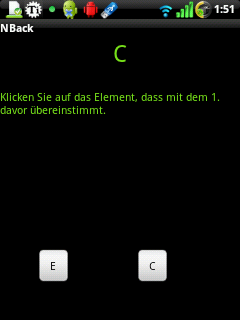
\includegraphics[width=0.4\linewidth]{pictures/screenshot-nback}
	\caption{Screenshot des n-back Test, aufgenommen von einem HTC Wildfire}
	\label{fig:sreen-nback}
	\end{figure}	
\end{frame}
\begin{frame}
	\begin{table}[htbp]

	    \begin{center}
	        \begin{footnotesize}
	            \begin{tabularx}{\linewidth}{l X}
	                \textbf{Parameter} & \textbf{Bedeutung}\\
	                \hline
	                n & Anzahl der Elemente vorher, auf die sich die Aufgabenstellung bezieht\\
	                displayTime & Anzeigedauer des dargestellten Wertes\\
	                length & Anzahl der Werte, die präsentiert werden\\
	                displayValues & Anzahl der Buttons, die sichtbar gemacht werden sollen \\
	                numberDigets & legt fest, ob Zahlen statt Buchstaben gezeigt werden sollen
	                
	            \end{tabularx}
	        \end{footnotesize}
	        
	        \label{tbl:paramNBack}
	    \end{center}
	    
	\end{table}
\end{frame}